In this section, we consider the $2\pi$-periodic Cauchy problems
\begin{align*}
u_t &= \alpha u_{xx} + \beta u_{xxxx} \\
u(x,0) &= sin(x)
\end{align*}


\subsection{Well-posed for $\alpha>0$ and $\beta = 0$}
We now show that the problem is well-posed in the $L_2$ -norm for for $\alpha>0$ and $\beta = 0$, i.e.
\begin{align*}
u_t &= \alpha u_{xx} \\
u(x,0) &= sin(x) = f(x)
\end{align*} 

To show well-posedness we need to show that a solution exists, is unique and is stable in some sense. According to the task, we assume existence. First we show uniqueness of this solution. So assume we have two solutions, $u_1$ and $u_2$. Then $u_1$ and $u_2$ satisfy
\begin{align*}
(u_1)_t &= \alpha (u_1)_{xx}\\ 
(u_2)_t &= \alpha (u_2)_{xx}\\
u_1(x,0) &= sin(x)\\
u_2(x,0) &= sin(x)
\end{align*}

Let us define $w=u_1-u_2$. Subtracting the equations together, we have that : 
\begin{align*}
(u_1)_t-(u_2)_t & = \alpha ((u_1)_{xx}-(u_2)_{xx})\\ 
u_1(x,0)-u_2(x,0) &= sin(x)-sin(x)=0
\end{align*}

Because of the linearity of the derivative operator, we have that $w$ is the solution of :
\begin{align*}
w_t & = \alpha w_{xx}\\ 
w(x,0) &= 0
\end{align*}

It is easy to see that the only solution to this problem is $w(x,t) = 0$ so we can conclude that the solution is unique because :
$$w=u_1-u_2 = 0 \implies u_1 = u_2$$

Let us now show stability. To do this we will compute the time derivative of the $L_2$ norm of the solution.
\begin{align*}
\frac{d}{dt} ||u(\cdot,t)||^2_{L_2} &= 2\int_0^{2\pi} u u_t dx \\
&=2\alpha \int_0^{2\pi} u u_{xx} dx\\
&=2\alpha ([uu_x]^{2\pi}_0 - \int_0^{2\pi} u_x u_x dx)
\end{align*}

Where we first used the PDE then integration by part.

By periodicity of the solution, we have that :
$$[uu_x]^{2\pi}_0 = u(2\pi,t)u_x(2\pi,t) - u(0,t)u_x(0,t) = 0$$
$$\frac{d}{dt} ||u(\cdot,t)||^2_{L_2}  = -2\alpha \int_0^{2\pi} (u_x)^2 dx \leq 0$$

Because the $L_2$ norm is decreasing, this allows us to conclude that : 
$$ ||u(\cdot,t)||^2_{L_2} \leq ||f||^2_{L_2}$$

We thus have stability and the problem is well-posed.

\subsection{Ill-posed for $\beta>0$}
To show ill-posedness, we need to find a family of solutions with the same $L_2$ norm initially whose growth rate is unbounded. Let us define the problem $P_k$ (for $k=1,2,...$) in the following way :
\begin{align*}
u_t &= \alpha u_{xx} + \beta u_{xxxx}\\
u(x,0) &= f_k(x) = sin(kx)
\end{align*}

Let us first compute the $L_2$ norm of the initial data : 
$$||f_k||^2_{L_2} = \int_0^{2\pi} sin^2(kx)dx=\int_0^{2\pi} \frac{1-cos(2kx)}{2}dx=\pi = ||f||^2_{L_2}$$ 

So all these initial data have the same norm. We can also easily see that the solution of $P_k$ is given by :
$$u(x,t) = sin(kx)e^{(-k^2\alpha + k^4\beta)t}$$ 

Because $\beta > 0$, we note that for sufficiently large $k$, increasing $k$ increases the growth rate of the solution. To show this, let us try and compute the $L_2$ norm of the solution.
$$||u(\cdot,t)||_{L_2}^2=\int_0^{2\pi} sin^2(kx)e^{2(-k^2\alpha + k^4\beta)t}dx= e^{2(-k^2\alpha + k^4\beta)t}\int_0^{2\pi} sin^2(kx)dx = e^{2(-k^2\alpha + k^4\beta)t} ||f||^2_{L_2} $$

Because $k$ can be as large as we want and because $\beta > 0$, it is not possible to bound this by an expression of the form $Ce^{mt}||f||$ where $C$ and $m$ do not depend on the initial data (and thus $k$). We can therefore conclude that the problem is ill-posed. 

\subsection{Max norm stability for $\alpha>0$ and $\beta=0$}
We wish to derive a condition on $\Delta t$ which guarantees stability in the max norm for a scheme using central difference in space and forward Euler in time. Our scheme is thus
\begin{align*}
\frac{u_j^{n+1} - u_j^n}{\Delta t}&=\alpha \frac{u_{j+1}^n -2u_j^n+u_{j-1}^n}{\Delta x^2} \\
\implies u_j^{n+1} &= u_j^n + \frac{\alpha \Delta t}{\Delta x^2} (u_{j+1}^n -2u_j^n+u_{j-1}^n) \\
&=  \frac{\alpha \Delta t}{\Delta x^2} (u_{j+1}^n +u_{j-1}^n) + (1-2\frac{\alpha \Delta t}{\Delta x^2})u_j^n 
\end{align*}
We see that for $\frac{\alpha \Delta t}{\Delta x^2} \in [0,\frac{1}{2}]$ that $u_j^{n+1}$ is a weighted average of $u_{j-1}^n,u_j^n$ and $u_{j+1}^n$ ($\frac{\alpha \Delta t}{\Delta x^2}$ weight for $u_{j+1}^n$ and $u_{j-1}^n$ and $1-2\frac{\alpha \Delta t}{\Delta x^2}$ for $u_j^n$).
This implies that
\begin{align}
|u_j^{n+1}| \leq \max(|u_{j-1}^n|,|u_j^n|,|u_{j+1}^n|) \qquad \forall j \label{maxeq} \\
\implies \max_j (|u_j^{n+1}|) \leq \max_j (|u_j^{n+1}|) \nonumber
\end{align}

We quickly note that if $\frac{\alpha \Delta t}{\Delta x^2}>\frac{1}{2}$, then it is possible to pick $u_{j-1}^n,u_j^n,u_{j+1}^n$ such that (\ref{maxeq}) is not fulfilled. Therefore are stability criterion is 
\begin{align*}
\frac{\alpha \Delta t}{\Delta x^2} &\leq \frac{1}{2} \\
\Delta t &\leq \frac{\Delta x^2}{2\alpha}
\end{align*}

\subsection{Max norm stability for $\beta \neq 0$}
The second order finite difference for the fourth order derivative is given by:
$$u_{xxxx} \approx \frac{u_{j+2}-4u_{j+1}+6u_j-4u_{j-1}+u_{j-2}}{\Delta x^4}$$

That gives us the following scheme : 
\begin{align*}
u_j^{t+1} &= u_j^t + \alpha\frac{\Delta t}{\Delta x^2} (u_{j+1}^t-2u_j^t+u_{j-1}^t)+ \beta \frac{\Delta t}{\Delta x^4}(u_{j+2}^t-4u_{j+1}^t+6u_j^t-4u_{j-1}^t+u_{j-2}^t)
\end{align*}

If we pose $\lambda = \alpha\frac{\Delta t}{\Delta x^2}$ and $\gamma = \beta \frac{\Delta t}{\Delta x^4}$, we have the following method : 
$$u_j^{t+1} = (1-2\lambda+6\gamma)u_j^t + \gamma u_{j+2}^t + \gamma u_{j-2}^t + (\lambda - 4\gamma)u_{j+1}^t + (\lambda - 4\gamma)u_{j-1}^t$$

We note that the sum of the coefficients is 1 so if all the coefficients are between 0 and 1, we have a weighted average and the conclusion derived for the case $\beta = 0$ holds. This is a rather complex system of inequalities. Figure \ref{reg} shows the region where $\lambda$ and $\gamma$ yield a stable method in max norm. The region is in red. Let us already note that we have a feasible region but this region depends on the value of $\alpha$ and $\beta$ so it is possible that for certain values, we cannot find a stable discretization. Furthermore, $N\Delta x=2\pi$ where $N$ must be an integer. That could also prove impossible to fulfill in the region for given values of $\alpha$ and $\beta$. Different tests will be conducted further in this report.

\begin{figure}
\begin{center}
\includegraphics[scale=0.4]{reg.eps}
\caption{Stable $\lambda$ and $\gamma$}
\label{reg}
\end{center}
\end{figure}




\subsection{Von Neumann Analysis for the well-posed case}
For this case, we have $\beta = 0$ and $\alpha>0$. The method (derived above), with $\lambda = \alpha \frac{\Delta t}{\Delta x^2}$, is given by :
$$u_j^{t+1} = (1-2\lambda)u_j^t+\lambda u_{j+1}^t + \lambda u_{j-1}^t$$

We will use the following ansatz for the Von Neumann analysis (comes from Fourier analysis):
$$u_j^t = U^te^{ikX_j}$$

Plugging this ansatz in our method and because we have a uniform spatial grid : 
$$U^{t+1}e^{ikX_j} = (1-2\lambda)U^te^{ikX_j} + \lambda U^t e^{ik(X_j+\Delta x)}+ \lambda U^t e^{ik(X_j-\Delta x)}$$

Dividing by $U^t e^{ikX_j}$ on each side gives us the amplification factor :
\begin{align*}
\frac{U^{t+1}}{U^t} &= 1-2\lambda + \lambda (e^{ik\Delta x} + e^{-ik\Delta x})\\
&= 1-2\lambda +2\lambda cos(k\Delta x)\\
&= 1 + 2\lambda (cos(k\Delta x) -1)
\end{align*}

For the method to be stable, we want $|\frac{U^{t+1}}{U^t}| \leq 1$. So, we have :
\begin{align*}
-1 &\leq 1 + 2\lambda (cos(k\Delta x) -1) \leq 1\\
-2 &\leq 2\lambda (cos(k\Delta x) -1) \leq 0\\
-1 &\leq \lambda (cos(k\Delta x) -1) \leq 0\\
\end{align*}

Because $cos(k\Delta x) -1$ is always negative, the second inequality is fulfilled if and only if $\lambda \geq 0$. That is always the case since $\alpha >0$. For the first inequality, we have to consider the "worst" case. It happens when $cos(k\Delta x) = -1$ and then we need : 
$$-1 \leq -2 \lambda \implies \lambda \leq \frac{1}{2} $$

We see that we find back the same relation as before. In conclusion : 
$$0 \leq \alpha \frac{\Delta t }{\Delta x^2} \leq \frac{1}{2}$$

That is particularly restrictive. Indeed, dividing the spatial step by 2 forces us to have 4 times the number of points in the time discretization to keep stability.

\subsection{Von Neumann Analysis for the ill-posed case}
In this case, $\beta > 0$. Let us use the same technique. The method when $\beta$ is not zero is the one described in section 1.4 : 

$$u_j^{t+1} = (1-2\lambda+6\gamma)u_j^t + \gamma u_{j+2}^t + \gamma u_{j-2}^t + (\lambda - 4\gamma)u_{j+1}^t + (\lambda - 4\gamma)u_{j-1}^t$$

Where  $\lambda = \alpha\frac{\Delta t}{\Delta x^2}$ and $\gamma = \beta \frac{\Delta t}{\Delta x^4}$.

Let us plug the ansatz in this method and compute the amplification factor.
\begin{align*}
U^{t+1}e^{ikX_j} = &(1-2\lambda+6\gamma)U^{t}e^{ikX_j} + \gamma U^te^{ik(X_j+2\Delta x)}+ \gamma U^te^{ik(X_j-2\Delta x)}+...\\
&...(\lambda - 4\gamma) U^te^{ik(X_j+\Delta x)}+(\lambda - 4\gamma) U^te^{ik(X_j+\Delta x)}
\end{align*}

Dividing each side by $U^{t}e^{ikX_j}$ and using Euler's formula for the complex exponentials, we have :
\begin{align*}
\frac{U^{t+1}}{U^t} &= (1-2\lambda+6\gamma) + \gamma (e^{2ik\Delta x}+e^{-2ik\Delta x})+(\lambda - 4\gamma)(e^{ik\Delta x}+e^{-ik\Delta x})\\
&=(1-2\lambda+6\gamma) + 2\gamma cos(2k\Delta x) + 2(\lambda - 4\gamma)cos(k\Delta x)
\end{align*}

This is a rather complex expression and it is not clear which values yield a stable method. That is why we have implemented a matlab program that computes the amplification factor for every values of $\lambda$ and $\gamma$. The code is available at the end of the report. Figure \ref{reg2} shows the results, the area in blue is stable and the one in red is not.

\begin{figure}
\begin{center}
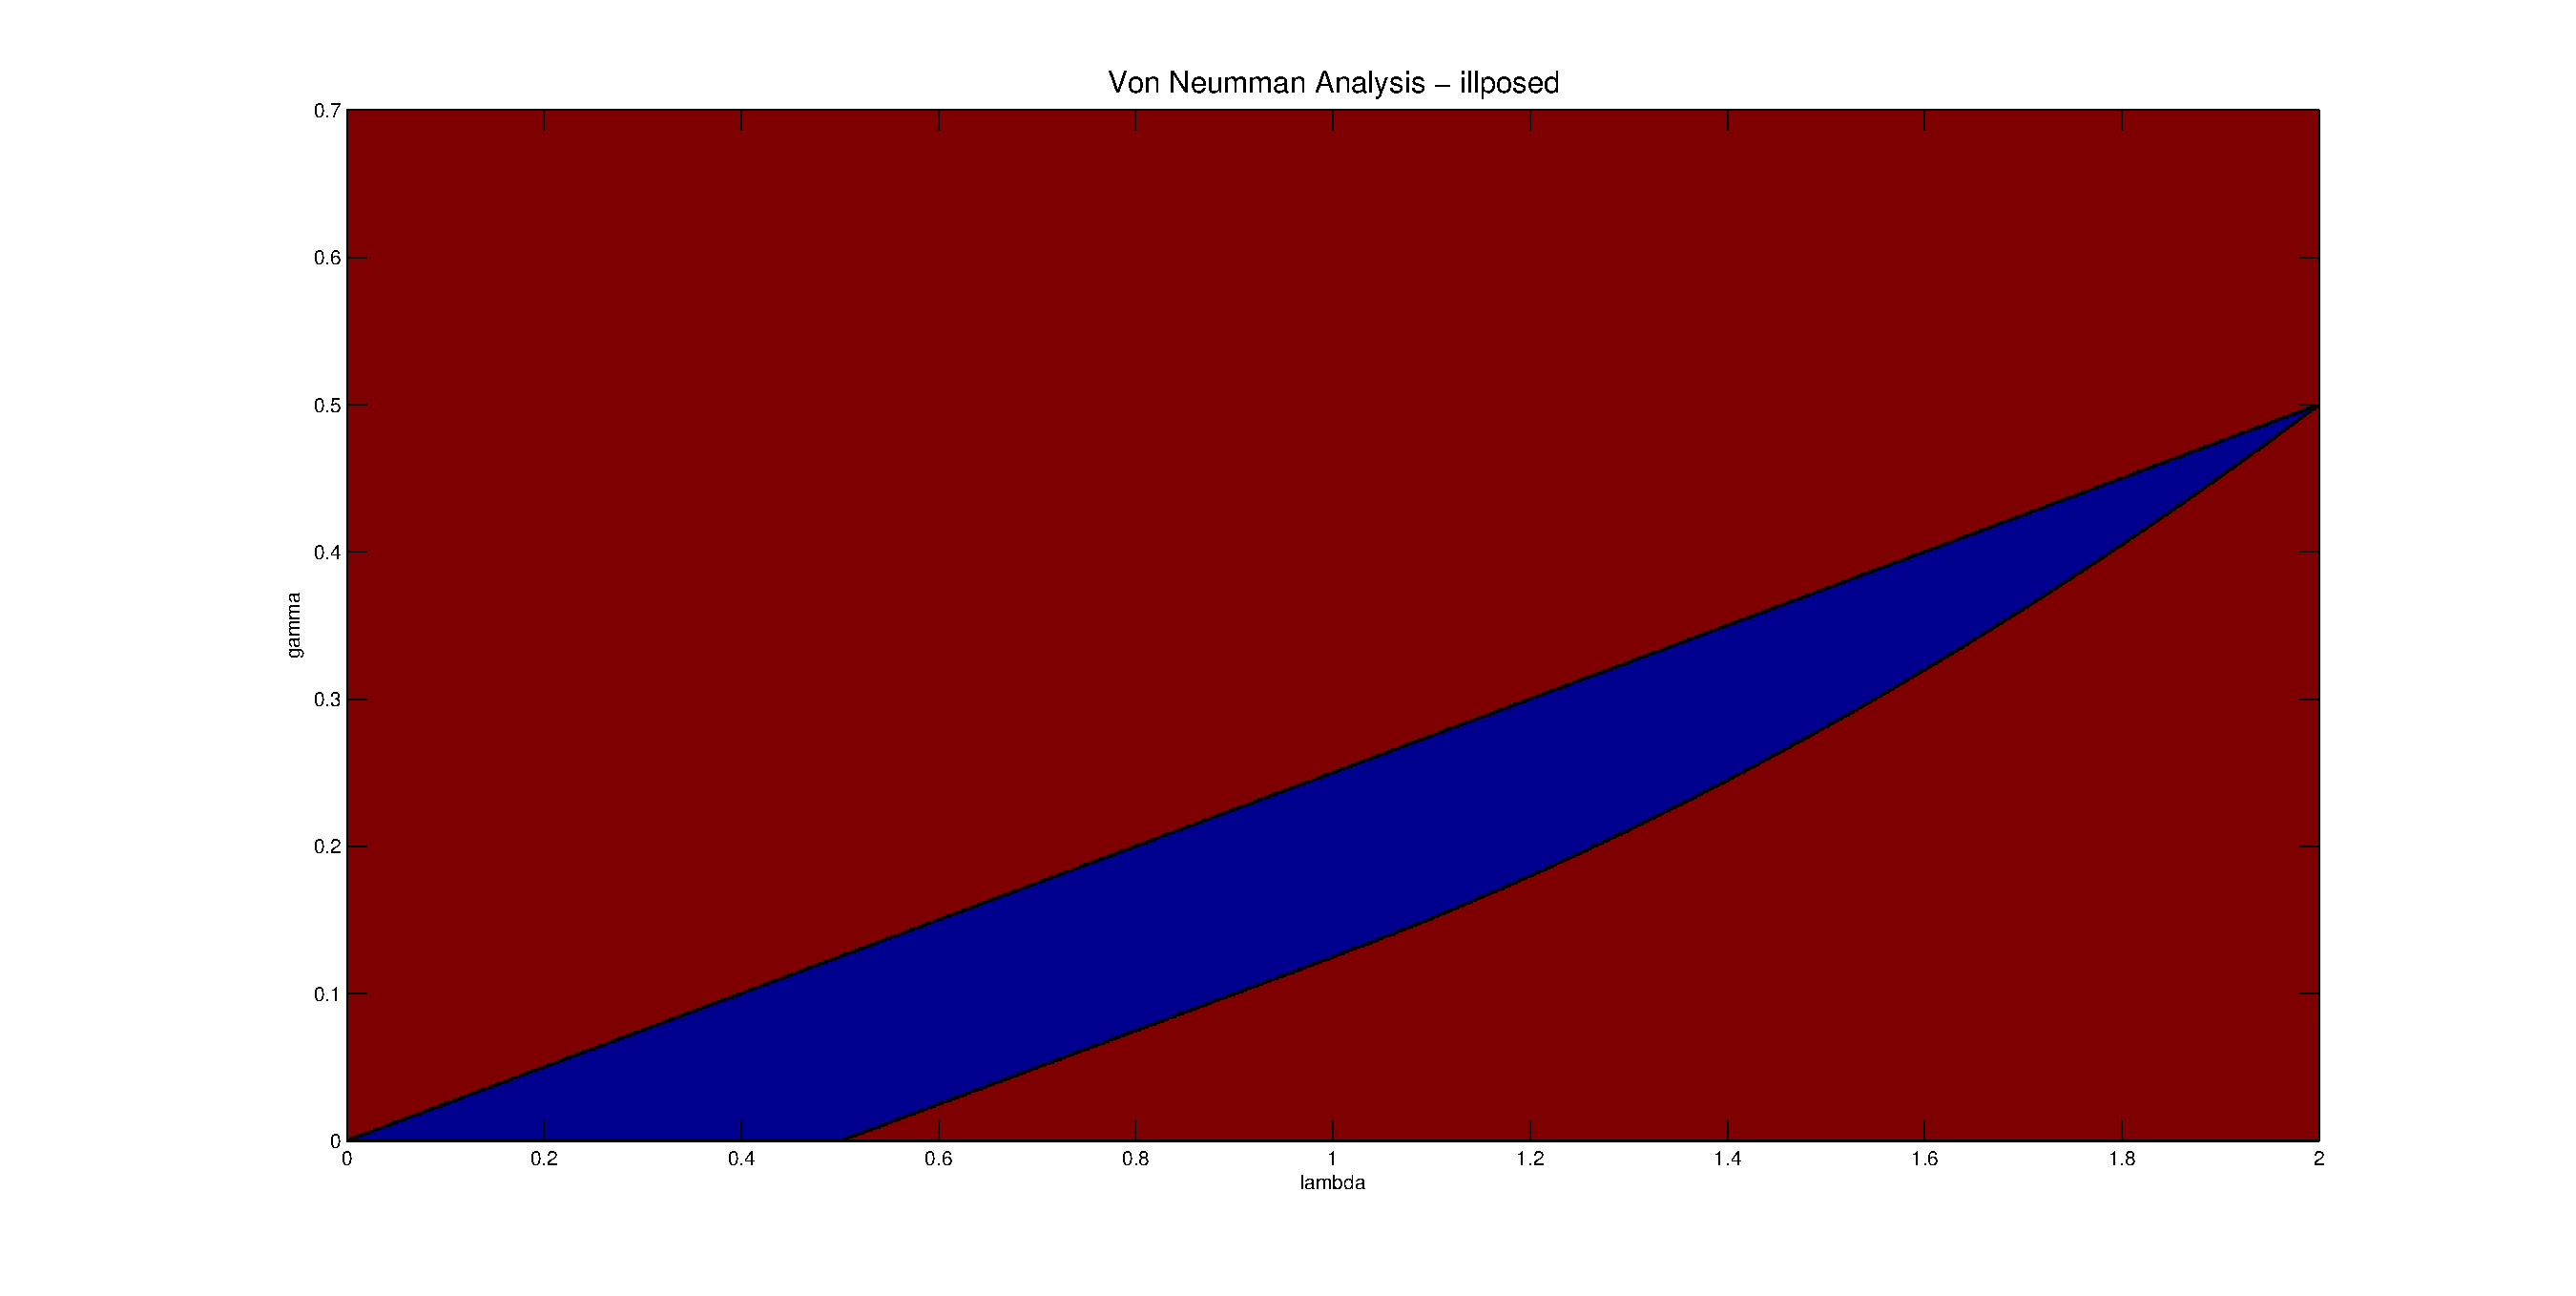
\includegraphics[scale=0.4]{reg2.eps}
\caption{Von Neumann analysis - illposed}
\label{reg2}
\end{center}
\end{figure}

The blue region is very similar to the one computed for the stability in max norm and the same remarks apply. So to answer the question, it is sometimes possible (provided that the given values of $\alpha$ and $\beta$ allow it) to have a stable discretization when $\beta \neq 0$. This will be checked in the next section.

\subsection{Proof through Numerical Experimentation}
The matlab code implementing the general scheme can be found at the end of the report and is called $diffu.m$.

Let us first test the first result : the fact that when $\beta = 0$, we need to have $\lambda \leq 0.5$ to have stability. Let us pose $N\Delta x = 2\pi$. Here, we used the following values : 
$$\alpha = \frac{(2\pi)^2}{2}$$
$$\Delta t = \frac{1}{2500}$$
$$ N \in \{30,40,50,51\}$$

Figure \ref{plot1} shows the numerical solution for different values of $\lambda$. We can easily see that the method is stable when $\lambda \leq 0.5$. The last plot, where $\lambda$ is slightly more than 0.5 shows instability so our results hold.

\begin{figure}
\begin{center}
\includegraphics[scale=0.4]{plot1.eps}
\caption{Numerical solution for different $\lambda$}
\label{plot1}
\end{center}
\end{figure}

Let us now move to the more complex part and make tests when $\beta \neq 0$. For this part, we have tried different values inside and outside the region given in figure \ref{reg}. The four dots represents the four discretization used. Figure \ref{plot2} shows the results.

\begin{figure}
\begin{center}
\includegraphics[scale=0.4]{plot2.eps}
\caption{Numerical solution for different $\lambda$ and $\gamma$}
\label{plot2}
\end{center}
\end{figure}

For the first three plots, we have used the following numerical value : 
$$\alpha = (2\pi)^2$$
$$\beta = \frac{(2\pi)^4}{60000}$$
$$\Delta t = \frac{1}{20000}$$

The first plot is the blue point (see figure \ref{reg}) which is located in $\lambda = 0.5$ and $\gamma = 0.0833$ ($N=100$). That is in the stable region and the numerical solution is stable. The second plot is the black point. It is located in $\lambda = 0.72$ and $\gamma = 0.1728$ ($N=120$). It is closer to the edge but still in the stable region and the numerical solution is stable.

Let us now talk about the two last plots. The third (the green one) is unstable and so is the numerical solution. It is located in $\lambda = 0.7812$ and $\gamma = 0.2035$ ($N=125$). For the last one, we wanted a point that was under the region so we changed $\beta$. For the last plot, $\beta = 0.0093$. We also have $N=180$ which gives : $\lambda = 1.62$ and $\gamma = 0.3124$. The point (in pink) is not in the stable region and the numerical solution is not stable.

In conclusion, the experiments conducted seem to confirm the analytic results.

